\documentclass[12pt]{article}

\usepackage{fullpage}
\usepackage[spanish]{babel}
\usepackage{amsfonts} %for double trace letters
\usepackage{amssymb}
\usepackage{amsmath} %for special/unusual mathematical characters
\usepackage{eufrak} %for gothic letters
\usepackage{graphicx} %Image includer package
\graphicspath{{Images/}} %Image directory
\usepackage{xcolor}

\usepackage{multicol} %For writing text in columns
\setlength{\columnsep}{1cm} %Defines separation of columns

\usepackage{tcolorbox} %for boxes that enclose text
\usepackage{color}
\definecolor{myblue}{rgb}{.8, .8, 1}

\usepackage{empheq}

\newlength\mytemplen
\newsavebox\mytempbox

\makeatletter
\newcommand\mybluebox{%
    \@ifnextchar[%]
       {\@mybluebox}%
       {\@mybluebox[0pt]}}

\def\@mybluebox[#1]{%
    \@ifnextchar[%]
       {\@@mybluebox[#1]}%
       {\@@mybluebox[#1][0pt]}}

\def\@@mybluebox[#1][#2]#3{
    \sbox\mytempbox{#3}%
    \mytemplen\ht\mytempbox
    \advance\mytemplen #1\relax
    \ht\mytempbox\mytemplen
    \mytemplen\dp\mytempbox
    \advance\mytemplen #2\relax
    \dp\mytempbox\mytemplen
    \colorbox{myblue}{\hspace{1em}\usebox{\mytempbox}\hspace{1em}}}

% for theorems
\usepackage{amsthm}
 
\theoremstyle{definition}
\newtheorem{definition}{Definici\'on}[section]


\begin{document}
	\title{Regiones en el Plano Complejo}
	\author{Breggia, Bruno M.}
	\date{}
	\maketitle
	
El Plano de Argand, o Plano Complejo, es un plano de extensi\'on infinita, pero no tenemos por qu\'e asustarnos, conocemos ya planos de ese estilo, como $\mathbb{R}^2$. \'Este, sin embargo, nos esconde muchas sorpresas nuevas. Para adentrarnos a este laberinto de sorpresas que encierra $\mathbb{C}$, debemos estudiarlo meticulosamente, parte por parte. Es zambullirnos a una pileta de definiciones nuevas y abstracciones. As\'i que p\'onganse las antiparras y aguanten la respiraci\'on.
\linebreak
	
\begin{center}
	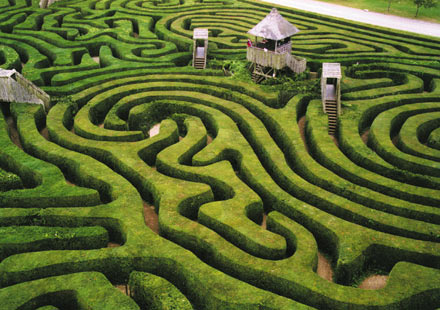
\includegraphics[scale=0.8]{laberinto.jpg}
\end{center}

\pagebreak
\tableofcontents
\pagebreak

\section{Conjuntos y elementos, un repaso}

\colorbox{red!40!white!80}{\parbox{\linewidth}{
\theoremstyle{definition}
\begin{definition} Conjuntos

Un conjunto es una agrupaci\'on bien definida de objetos. Esos objetos pueden ser n\'umeros, letras, personas, otros conjuntos, etc.

\end{definition}}}
\linebreak

Los conjuntos se denotan con letra may\'uscula, y los objetos que lo componen se denominan \textbf{elementos}.\\

\colorbox{red!40!white!80}{\parbox{\linewidth}{
\theoremstyle{definition}
\begin{definition} Pertenencia

Si un elemento $x$ forma parte de un cojunto $A$, diremos que el elemento $x$ \textbf{pertenece} a $A$, y se denota mediante: $$x \in A$$
En caso contrario, diremos que $x$ \textit{no pertenece} a $A$, y se escribe: $$x \notin A$$

\end{definition}}}\\
\linebreak

Hay dos maneras de anotar conjuntos:
\begin{itemize}
	\item Por \textbf{comprensi\'on}: cuando se describe una propiedad que caracteriza a todos sus elementos. $$A = \{x\: :\: x \hbox{ cumple cierta condici\'on} \}$$
	\item Por \textbf{extensi\'on}: se listan cada uno de sus elementos expl\'icitamente. $$A = \{x_1, x_2, x_3, ... \}$$
\end{itemize}

\subsection{Igualdad de Conjuntos}
Diremos que dos conjuntos son \textbf{iguales} si y s\'olo si ambos est\'an formados por los mismos elementos.

\begin{empheq}[box={\mybluebox[5pt]}]{equation*}
	\mbox{ \large $ A=B \Leftrightarrow \forall x \in A \rightarrow x \in B \land \forall x \in B \rightarrow x \in A$}
\end{empheq}
\linebreak

La igualdad de conjuntos presenta las siguientes propiedades:
\begin{itemize}
	\item \textbf{Reflexiva}: todo conjunto es igual a s\'i mismo.
	\item \textbf{Simetr\'ia}: $A=B \Leftrightarrow B=A$
	\item \textbf{Transitiva}: Si $A=B \land B=C \Rightarrow A=C$
\end{itemize}

\subsection{Subconjuntos}
Se dice que $A$ es un \textbf{subconjunto} de $B$ si todos los elementos de $A$ tambi\'en son elementos de $B$. Si $A$ es un subconjunto de $B$, lo denotaremos como:
$$A \subset B$$

El conjunto que no contiene ning\'un elemento se llama \textbf{Conjunto Vac\'io}, y se denota por $\emptyset$. El conjunto vac\'io es \'unico, y \'este es subconjunto de todo conjunto.

De manera similar, diremos que el \textbf{Conjunto Universal} $U$ es el conjunto de \textit{todos} los elementos en el contexto en el cual estamos trabajando.

\begin{center}
	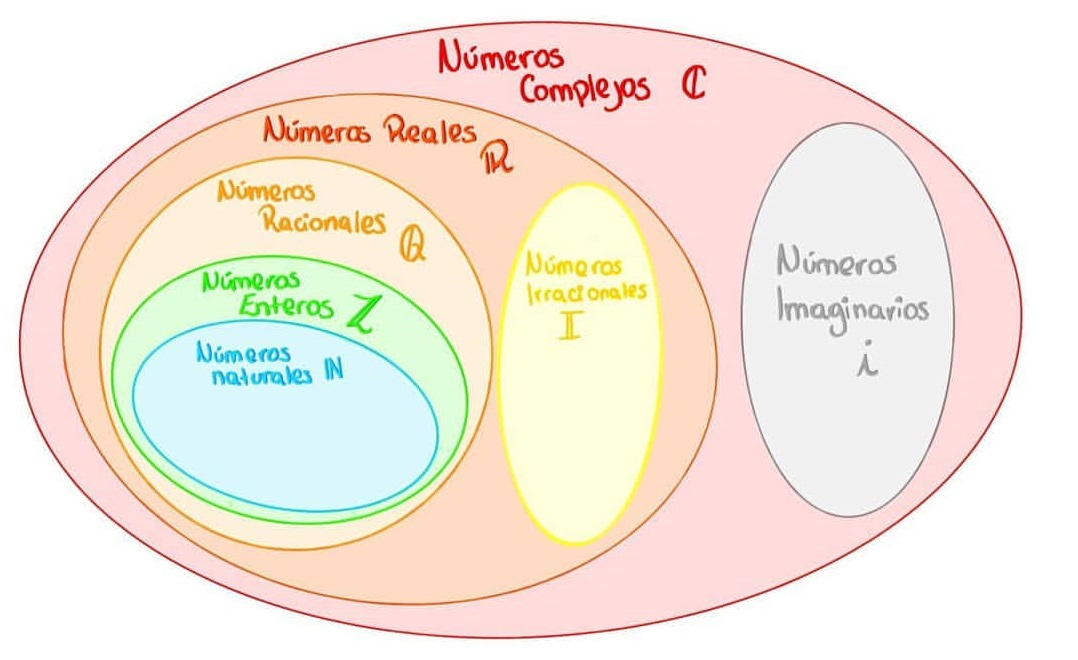
\includegraphics[scale=0.5]{conjuntos.jpg}
\end{center}

\subsection{Operaciones entre conjuntos}
Entre conjuntos vamos a definir las siguientes operaciones:
\begin{itemize}
	\item \textbf{Uni\'on}: la uni\'on entre dos conjuntos $A$ y $B$ se denota $A \cup B$ y es el conjunto de todos los elementos que pertenecen al menos a uno de los conjuntos $A$ y $B$.
	\item \textbf{Intersecci\'on}: la intersecci\'on entre dos conjuntos $A$ y $B$ se denota $A \cap B$ y es el conjunto de todos los elementos que pertenecen tanto a $A$ como a $B$.
	\item \textbf{Complemento}: el complemento de un conjunto $A$, que se denota por $A^C$, es el conjunto de todos los elementos que \textit{no} est\'an en $A$. De tal manera que la uni\'on de cualquier conjunto con su complemento es igual al conjunto universal, y la intersecci\'on es el conjunto vac\'io.
\end{itemize}

\section{Definiciones en el Plano de Argand}
Ahora volvemos a tierra y nos adentraremos espec\'ificamente en el conjunto $\mathbb{C}$, el conjunto de todos los n\'umeros complejos. Mucho nos espera por delante.\\

\colorbox{red!40!white!80}{\parbox{\linewidth}{
\theoremstyle{definition}
\begin{definition} Distancia entre N\'umeros Complejos

La distancia entre dos n\'umeros complejos $z_1, z_2$ se define como:
$$d(z_1, z_2) \triangleq |z_1 - z_2|$$
\end{definition}}}

\begin{multicols} {2}
\begin{eqnarray*}
d(z_1, z_2) &=& |z_1 - z_2|\\
&=& |(x_1 + iy_1) - (x_2+iy_2)|\\
&=& |(x_1-x_2) + i(y_1-y_2)|\\
&=& \sqrt[2]{(x_1-x_2)^2 + (y_1-y_2)^2}
\end{eqnarray*}
\linebreak

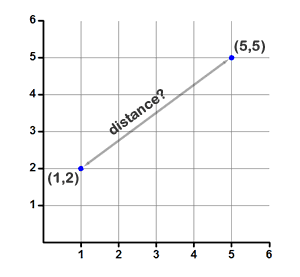
\includegraphics[scale=0.7]{distance.png}
\end{multicols}

\colorbox{red!40!white!80}{\parbox{\linewidth}{
\theoremstyle{definition}
\begin{definition} Circunferencia

Dados $z_0 \in \mathbb{C}$ y $\delta \in \mathbb{R}^+$, se define \textbf{circunferencia} de centro $z_0$ y radio $\delta$ al conjunto de $z \in \mathbb{C}$ tales que su distancia a $z_0$ sea $\delta$, es decir, que $d(z, z_0) = \delta$.

Expresaremos a la circunferencia $S$ simb\'olicamente de la siguiente manera:
$$ S(z_0, \delta) = \{ z \in \mathbb{C}\ :\ |z-z_0|=\delta \} $$
\end{definition}}}

%\begin{multicols} {2}
\begin{eqnarray*}
d(z, z_0) &=& \delta \\
\sqrt[2]{(x-x_0)^2 + (y-y_0)^2} &=& \delta\\
(x-x_0)^2 + (y-y_0)^2 &=& \delta^2\\
\end{eqnarray*}

Vemos que, trabajando con las partes real e imaginaria de los n\'umeros complejos, llegamos a la expresi\'on para una circunferencia en el plano $\mathbb{R}^2$, centrada en $(x_0, y_0)$ y de radio $\delta$.
\begin{center}
	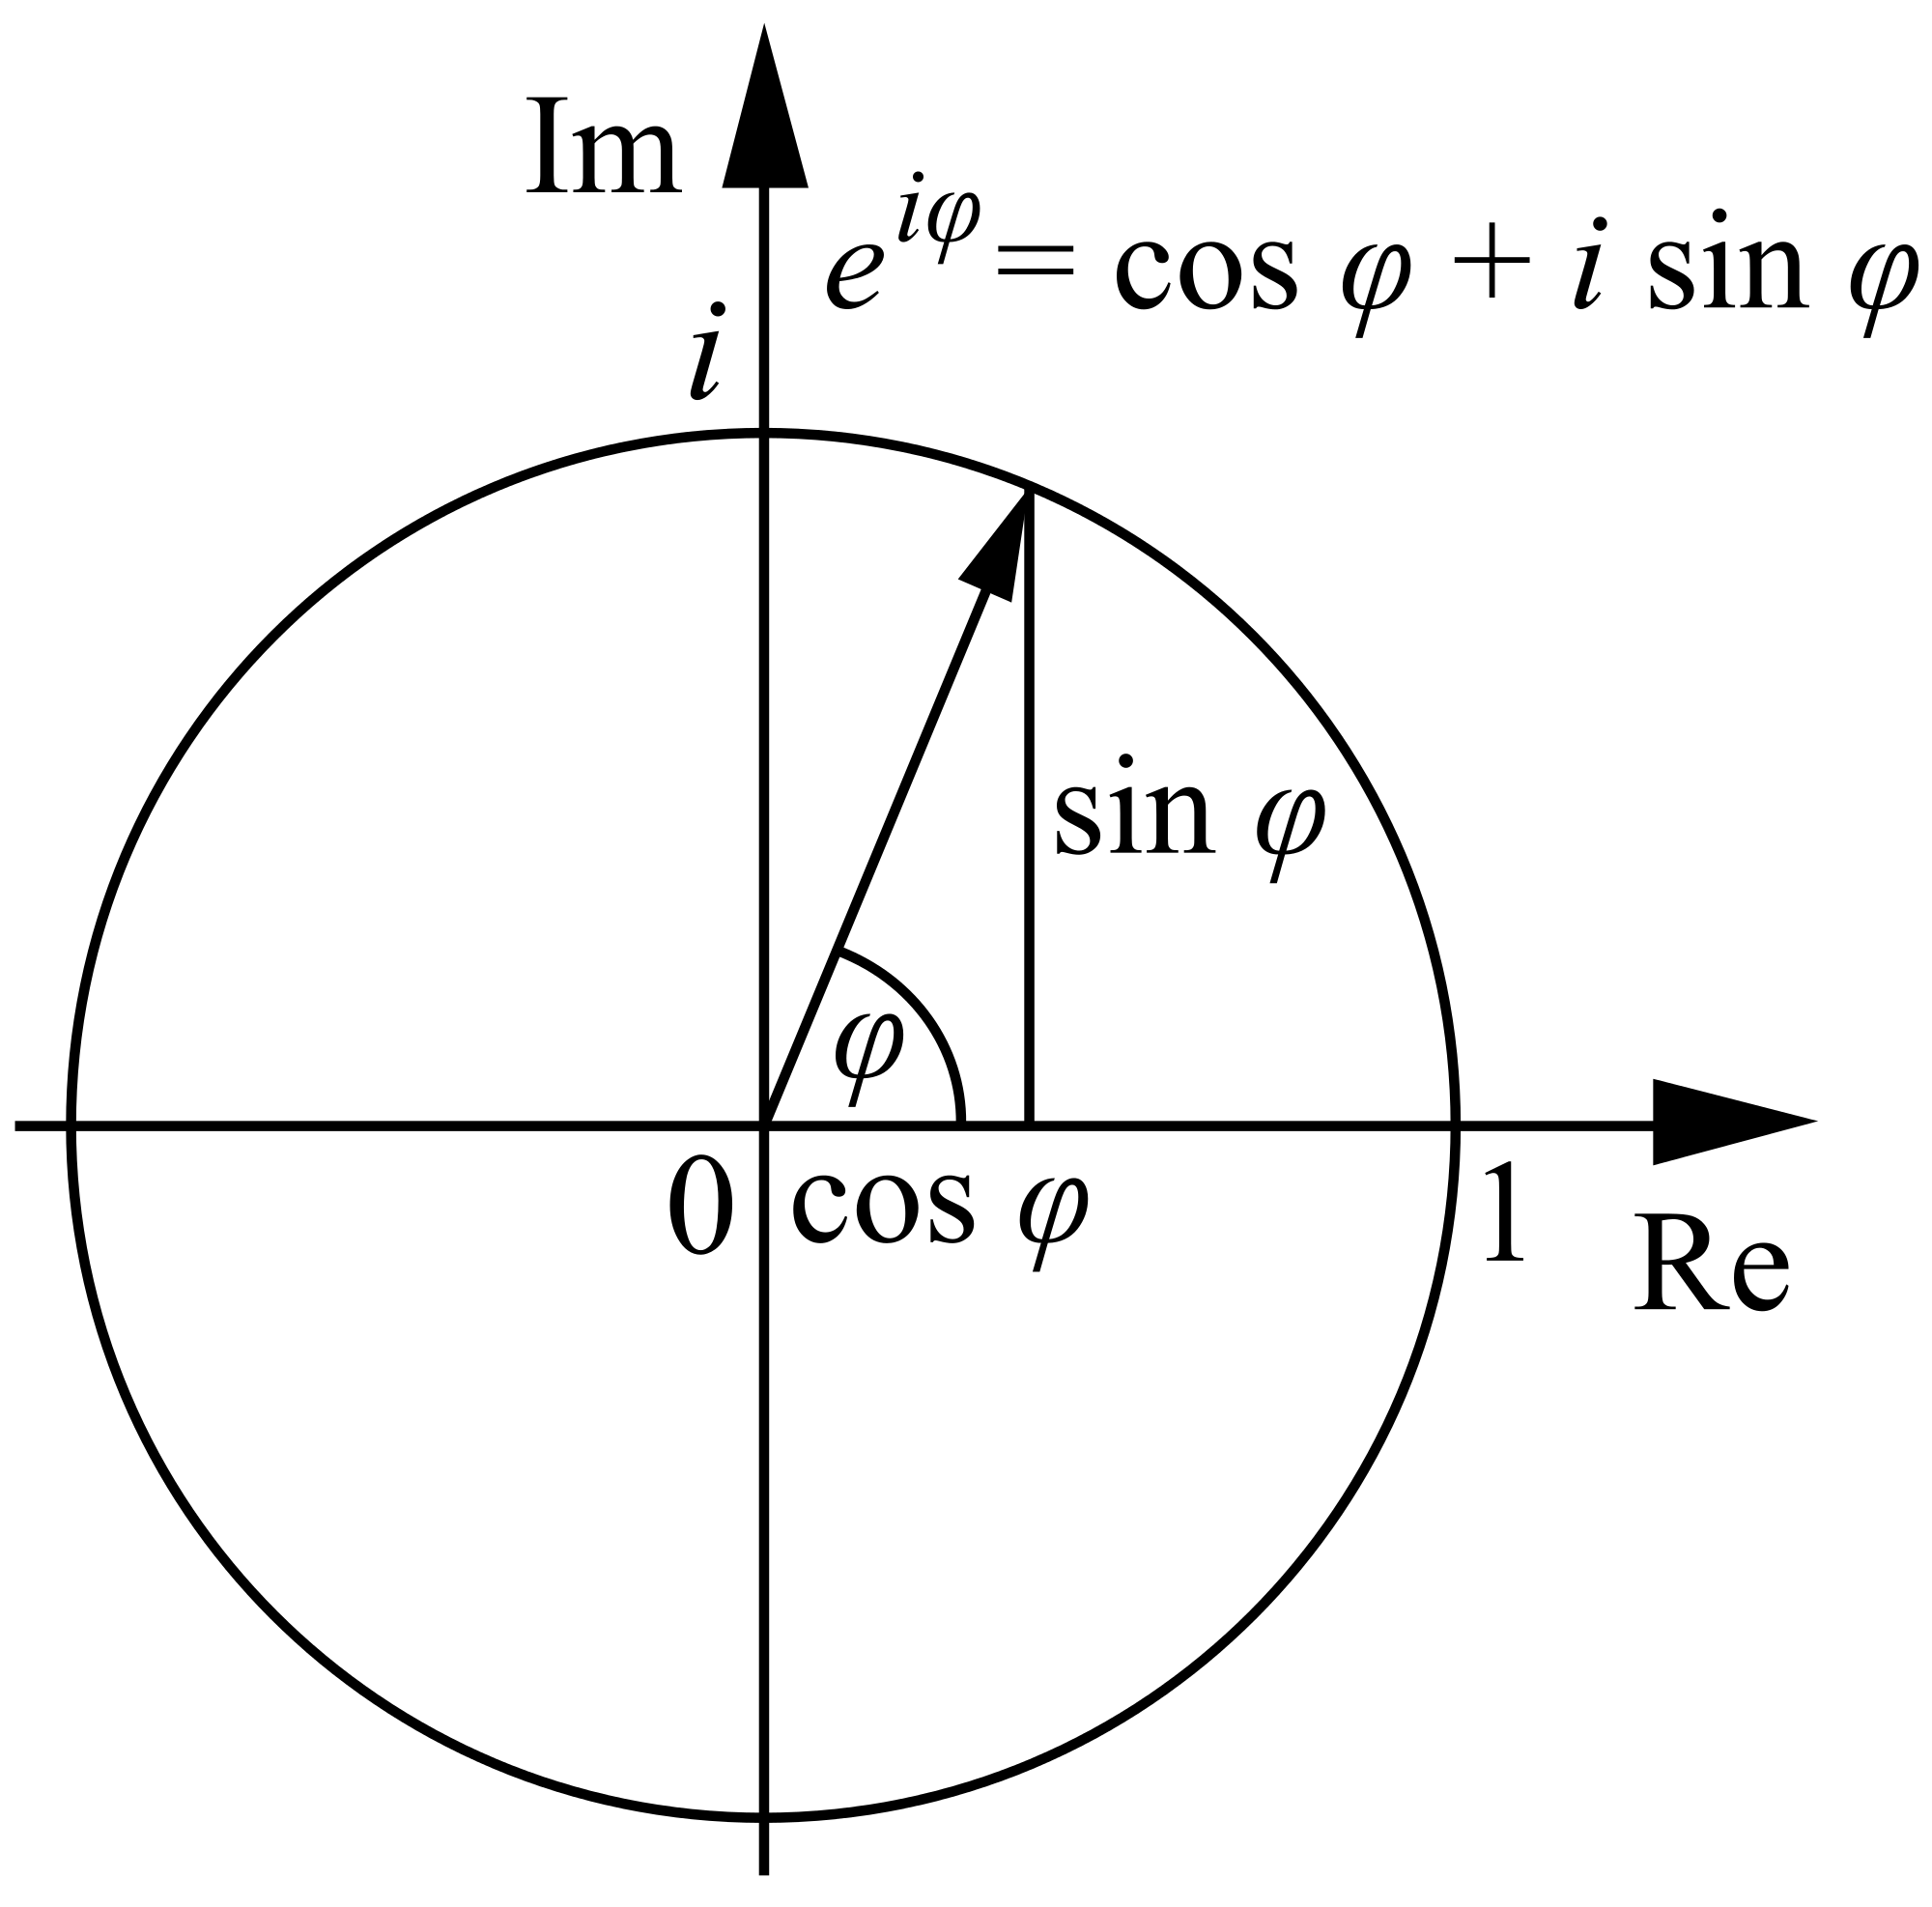
\includegraphics[scale=0.08]{circulo.png}
\end{center}
%\end{multicols}

\colorbox{red!40!white!80}{\parbox{\linewidth}{
\theoremstyle{definition}
\begin{definition} Entorno

Dados $z_0 \in \mathbb{C}$ y $\varepsilon \in \mathbb{R}^+$, se define \textbf{entorno} de centro $z_0$ y radio $\varepsilon$ al conjunto de $z \in \mathbb{C}$ tales que su distancia a $z_0$ sea menor a $\varepsilon$, es decir, que $d(z, z_0) < \varepsilon$.

Expresaremos al entorno $\eta$ simb\'olicamente de la siguiente manera:
$$ \eta(z_0, \varepsilon) = \{ z \in \mathbb{C}\ :\ |z-z_0|<\varepsilon\} $$
\end{definition}}}

\begin{multicols} {2}
\begin{eqnarray*}
d(z, z_0) &<& \varepsilon\\
\sqrt[2]{(x-x_0)^2 + (y-y_0)^2} &<& \varepsilon\\
(x-x_0)^2 + (y-y_0)^2 &<& \varepsilon^2\\
\end{eqnarray*}


\begin{center}
	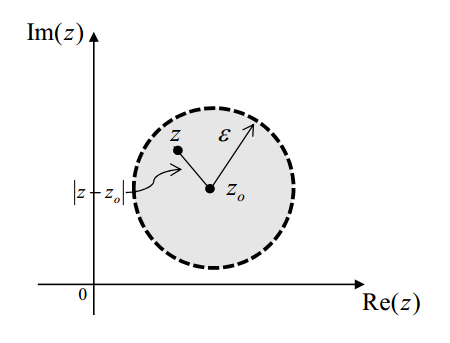
\includegraphics[scale=0.7]{entorno.png}
\end{center}
\end{multicols}

\colorbox{red!40!white!80}{\parbox{\linewidth}{
\theoremstyle{definition}
\begin{definition} Anillo o Corona

Dados $z_0 \in \mathbb{C}$ y $r_1, r_2 \in \mathbb{R}^+$ con $r_1<r_2$, se define \textbf{corona} o \textbf{anillo} de centro $z_0$ al conjunto de $z \in \mathbb{C}$ tales que su distancia a $z_0$ se encuentre entre $r_1$ y $r_2$.

Expresaremos al anillo $A$ simb\'olicamente de la siguiente manera:
$$ A(z_0,r_1, r_2) = \{ z \in \mathbb{C}\ :\ r_1 < |z-z_0| < r_2 \} $$
... o tambi\'en:
$$ A(z_0,r_1, r_2) = \{ z \in \mathbb{C}\ :\ r_1 \leq |z-z_0| \leq r_2 \} $$
\end{definition}}}

\begin{multicols} {2}
\begin{eqnarray*}
r_1 < &d(z, z_0)& < r_2\\
r_1 < &\sqrt[2]{(x-x_0)^2 + (y-y_0)^2}& < r_2\\
r_1^2 < &(x-x_0)^2 + (y-y_0)^2& < r_2^2\\
\\
r_1^2 \leq &(x-x_0)^2 + (y-y_0)^2& \leq r_2^2
\end{eqnarray*}
\linebreak

\begin{center}
	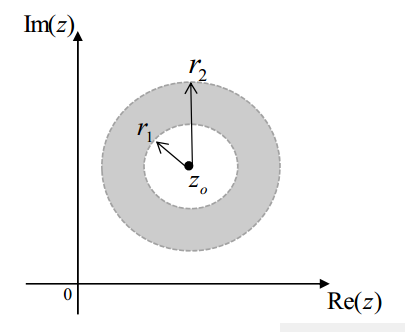
\includegraphics[scale=0.7]{corona.png}
\end{center}
\end{multicols}

\colorbox{red!40!white!80}{\parbox{\linewidth}{
\theoremstyle{definition}
\begin{definition} Entorno reducido

Dados $z_0 \in \mathbb{C}$ y $\varepsilon \in \mathbb{R}^+$, se define \textbf{entorno reducido} de centro $z_0$ y radio $\varepsilon$ al conjunto de $z \in \mathbb{C}$, con $z \neq z_0$ tales que su distancia a $z_0$ sea menor que $\varepsilon$. Tambi\'en se denomina entorno \textbf{perforado} o \textbf{punteado}, ya que su \'unica diferencia con un entorno propiamente dicho es que no incluye el complejo $z_0$ (el centro del entorno).

Expresaremos al entorno reducido $\eta^*$ simb\'olicamente de la siguiente manera:
$$ \eta^*(z_0, \varepsilon) = \{ z \in \mathbb{C}\ :\ 0<|z-z_0|<\varepsilon\} $$
\end{definition}}}

\begin{multicols} {2}
\begin{eqnarray*}
0<&d(z, z_0)& < \varepsilon\\
0<&\sqrt[2]{(x-x_0)^2 + (y-y_0)^2}& < \varepsilon\\
0<&(x-x_0)^2 + (y-y_0)^2& < \varepsilon^2\\
\end{eqnarray*}
%\linebreak

\begin{center}
	
\includegraphics[scale=0.25]{perforadora.jpg}
\end{center}

\begin{center}
	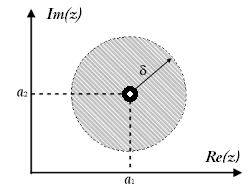
\includegraphics[scale=1.1]{entornoReducido.png}
\end{center}
\end{multicols}

\section{Clasificando Puntos}

Para avanzar m\'as en las nociones de conjuntos complejos y pertenencia, debemos tener en claro las distintas definiciones de puntos que a continuaci\'on se presentar\'an.

\colorbox{yellow!40!white!80}{\parbox{\linewidth}{
\theoremstyle{definition}
\begin{definition} Punto Interior

Sea $S$ un conjunto del plano complejo, $S \subset \mathbb{C}$ y $z_0 \in \mathbb{C}$. Se dice que $z_0$ es un \textbf{punto interior} de $S$ si existe un entorno de $z_0$ cuyos puntos sean todos de $S$.

Simb\'olicamente, $z_0$ es un punto interior de $S \subset \mathbb{C}$ si y s\'olo si:
$$\exists \varepsilon \in \mathbb{R}^+ : \eta(z_0, \varepsilon) \subset S$$
...o tambi\'en se lo puede expresar como:
$$\exists \varepsilon \in \mathbb{R}^+ : \forall z \in \eta(z_0, \varepsilon), z \in S$$
\end{definition}}}

\begin{center}
	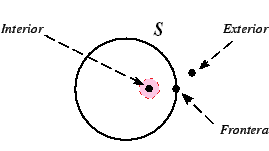
\includegraphics[scale=1]{pinterior.png}
\end{center}

\colorbox{yellow!40!white!80}{\parbox{\linewidth}{
\theoremstyle{definition}
\begin{definition} Punto Exterior

Sea $S$ un conjunto del plano complejo, $S \subset \mathbb{C}$ y $z_0 \in \mathbb{C}$. Se dice que $z_0$ es un \textbf{punto exterior} de $S$ si existe un entorno de $z_0$ que no contenga ning\'un punto de $S$.


Simb\'olicamente, $z_0$ es un punto exterior de $S \subset \mathbb{C}$ si y s\'olo si:
$$\exists \varepsilon \in \mathbb{R}^+ : \eta(z_0, \varepsilon) \cap S = \emptyset$$
...o tambi\'en se lo puede expresar como:
$$\exists \varepsilon \in \mathbb{R}^+ : \forall z \in \eta(z_0, \varepsilon), z \notin S$$
\end{definition}}}

\begin{center}
	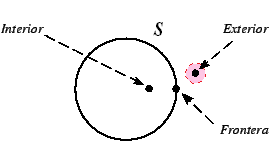
\includegraphics[scale=1]{pexterior.png}
\end{center}

\colorbox{yellow!40!white!80}{\parbox{\linewidth}{
\theoremstyle{definition}
\begin{definition} Punto Frontera

Sea $S$ un conjunto del plano complejo, $S \subset \mathbb{C}$ y $z_0 \in \mathbb{C}$. Se dice que $z_0$ es un \textbf{punto frontera} de $S$ si no es un punto interior ni punto exterior de $S$. Es decir, todo entorno con centro en $z_0$ tiene tanto puntos que pertenecen a $S$ como puntos que no.

Simb\'olicamente, $z_0$ es un punto frontera de $S \subset \mathbb{C}$ si y s\'olo si:
$$\forall \varepsilon \in \mathbb{R}^+ : \left( \exists z_1 \in \eta(z_0, \varepsilon) / z_1 \in S \right) \land \left( \exists z_2 \in \eta(z_0, \varepsilon) / z_2 \notin S \right)$$
...o tambi\'en se lo puede expresar como:
$$ \forall \varepsilon \in \mathbb{R}^+ : \eta(z_0, \varepsilon) \cap S \neq \emptyset \land  \eta(z_0, \varepsilon) \cap S^C \neq \emptyset $$
\end{definition}}}
\linebreak

\begin{center}
	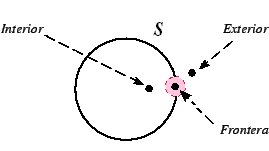
\includegraphics[scale=1]{pfrontera.png}
\end{center}


\texttt{OBSERVACI\'ON:} un punto frontera de un conjunto $S$ puede o no pertenecer al conjunto $S$. El que sea frontera no indica nada respecto a si est\'a incluido en el conjunto, sino s\'olo a su condici\'on f\'isica de delimitador del conjunto. Su inclusi\'on en el mismo estar\'a determinada por la forma en que se defina $S$.

\begin{multicols} {2}	
En una representaci\'on gr\'afica, si el contorno de un conjunto es una l\'inea s\'olida, incluye sus puntos frontera, si es una l\'inea punteada, no los incluye.

	\texttt{OBSERVACI\'ON:} al conjunto de los puntos frontera de un conjunto $S \subset \mathbb{C}$ se lo denomina \textbf{frontera} de $S$, y se lo denota como $\delta S$.\\
	\linebreak
	
	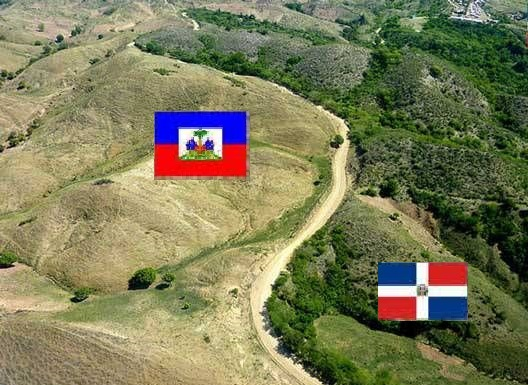
\includegraphics[scale=0.4]{frontera.jpg}
\end{multicols}

\colorbox{yellow!40!white!80}{\parbox{\linewidth}{
\theoremstyle{definition}
\begin{definition} Punto de Acumulaci\'on o Punto L\'imite

Sea $S$ un conjunto del plano complejo, $S \subset \mathbb{C}$ y $z_0 \in \mathbb{C}$. Se dice que $z_0$ es un \textbf{punto de acumulaci\'on} o \textbf{punto l\'imite} de $S$ si todo entorno centrado en $z_0$ contiene al menos un punto de $S$ distinto de $z_0$.

Simb\'olicamente, $z_0$ es un punto l\'imite de $S \subset \mathbb{C}$ si y s\'olo si:
$$\forall \varepsilon \in \mathbb{R}^+ : \eta^*(z_0, \varepsilon) \cap S \neq \emptyset$$
...o tambi\'en se lo puede expresar como:
$$ \forall \varepsilon \in \mathbb{R}^+ : (\exists z \in \eta(z_0, \varepsilon) / z \in S \land z \neq z_0) $$
\end{definition}}}
\linebreak

\begin{center}
	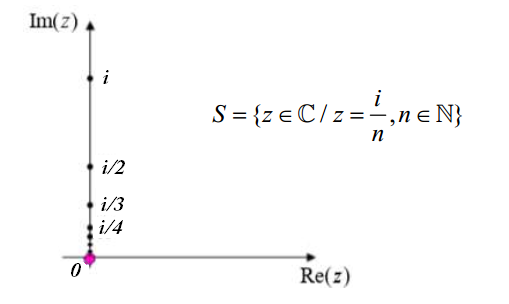
\includegraphics[scale=0.7]{acumulacion.png}
\end{center}

En el conjunto descripto en la imagen anterior, el punto $z=0$ es el \'unico punto de acumulaci\'on.

\section{Conjuntos en el Plano Complejo}
Ahora vamos a clasificar los conjuntos. Todo conjunto que se defina en el plano complejo de ahora en adelante deberemos catalogarlo seg\'un las clasificaciones que veremos a continuaci\'on: \\

\colorbox{green!40!white!80}{\parbox{\linewidth}{
\theoremstyle{definition}
\begin{definition} Conjunto Abierto

Sea $S \subset \mathbb{C}$. Se dice que $S$ es un \textbf{conjunto abierto} si no contiene ninguno de sus puntos frontera. Con ello, tenemos que todos sus puntos son interiores, o que $S$ es el conjunto vac\'io ($S = \emptyset$).

\end{definition}}}
\linebreak
\linebreak

\colorbox{green!40!white!80}{\parbox{\linewidth}{
\theoremstyle{definition}
\begin{definition} Conjunto Cerrado

Sea $S \subset \mathbb{C}$. Se dice que $S$ es un \textbf{conjunto cerrado} si contiene a \textit{todos} sus puntos frontera.

Tambi\'en podemos definirlo como sigue:
\begin{itemize}
	\item $S$ es cerrado si $S^C$ es un conjunto abierto.
	\item $S$ es cerrado si contiene a todos sus puntos de acumulaci\'on.
\end{itemize}

\end{definition}}}
\linebreak
\linebreak

\colorbox{green!40!white!80}{\parbox{\linewidth}{
\theoremstyle{definition}
\begin{definition} Clausura

Sea $S \subset \mathbb{C}$ un conjunto abierto. Se denomina \textbf{clausura} de $S$ al conjunto uni\'on de $S$ con su frontera. Se denota con $\overline{S}$.
$$\overline{S} = S \cup \delta S$$

\end{definition}}}
\linebreak

\begin{center}
	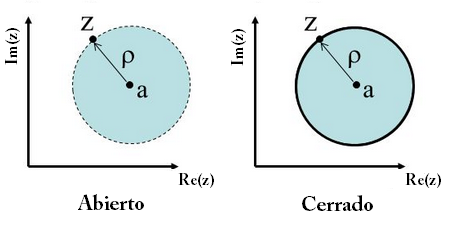
\includegraphics[scale=0.8]{tiposConjuntos.png}
\end{center}

\texttt{OBERVACI\'ON:} hay conjuntos en el plano complejo que no son abiertos ni cerrados (por ejemplo, si incluyen algunos de sus puntos frontera pero no a todos). Y tambi\'en pueden haber conjuntos que sean abiertos \textbf{y} cerrados, como todo el conjunto $\mathbb{C}$ en s\'i mismo.\\

\colorbox{green!40!white!80}{\parbox{\linewidth}{
\theoremstyle{definition}
\begin{definition} Conjunto Conexo

Sea $S \subset \mathbb{C}$. Se dice que $S$ es un \textbf{conjunto conexo} si y s\'olo si todo par de puntos de $S$ se pueden unir mediante una poligonal $C$ compuesto por la uni\'on de un n\'umero finito de segmentos rectos sucesivos, tal que $C$ est\'a \'integramente contenida en $S$.

\end{definition}}}
\linebreak
\linebreak

\colorbox{green!40!white!80}{\parbox{\linewidth}{
\theoremstyle{definition}
\begin{definition} Dominio Complejo

Un conjunto $S \subset \mathbb{C}$ abierto y conexo se denomina \textbf{dominio complejo.} 

\end{definition}}}
\linebreak
\linebreak

\colorbox{green!40!white!80}{\parbox{\linewidth}{
\theoremstyle{definition}
\begin{definition} Regi\'on en el Plano Complejo

Se denomina \textbf{regi\'on en el plano complejo} a la uni\'on de un dominio $S \subset \mathbb{C}$ con cualquier subconjunto de $\delta S$.

Es decir, es la uni\'on de $S$ con algunos, ninguno o todos sus puntos frontera.

\end{definition}}}
\linebreak

\begin{center}
	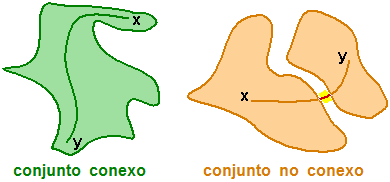
\includegraphics[scale=0.8]{conexidad.png}
\end{center}

\texttt{OBERVACI\'ON:} tenemos que todo entorno es un dominio, al no incluir su frontera, y ser conexo. A su vez, todo anillo es conexo, aunque no necesariamente es un dominio, ya que puede, o no, contener sus puntos frontera (puede no ser abierto).

De ambos casos mencionados, tenemos entonces que todo entorno es un dominio, mientras que s\'olo los anillos que sean abiertos lo ser\'an. \\

\colorbox{green!40!white!80}{\parbox{\linewidth}{
\theoremstyle{definition}
\begin{definition} Conjunto Acotado

Se dice que un conjunto $S \subset \mathbb{C}$ es \textbf{acotado} si existe un c\'irculo centrado en un $z_0 \in \mathbb{C}$ y de radio $R\in \mathbb{R}^+$ finito que lo contiene.

En caso de no cumplir con lo anterior, diremos que es \textbf{no acotado} (es de extensi\'on infinita).

\end{definition}}}
\linebreak
\linebreak

\colorbox{green!40!white!80}{\parbox{\linewidth}{
\theoremstyle{definition}
\begin{definition} Conjunto Compacto

Un conjunto $S \subset \mathbb{C}$ cerrado y acotado se dice que es un conjunto \textbf{compacto.} 

\end{definition}}}
\linebreak
\linebreak

\section{Recapitulando}
Llegados aqu\'i al final de la lecci\'on, se han visto muchos conjuntos y una inmensa cantidad de definiciones nuevas. Todo esto no es para agobiarnos, sino para adentrarnos de a poco, y de manera formal, en el concepto estrella de la disciplina: las \textit{funciones de variables complejas}. As\'i que tienen mi palabra, esto se pondr\'a \textbf{mejor}.

\begin{center}
	
\includegraphics[scale=0.6]{paradoja.jpg}\\
	\textit{?`El barbero... se afeita a s\'i mismo?}
\end{center}

\end{document}